\documentclass[twocolumn]{article}
\usepackage{amsmath}
\usepackage{amssymb}
\usepackage{graphicx}

\begin{document}


\section*{Simultaneous Linear Equations}

Method 1: Elimination

$
\begin{gathered}
	5 x-2 y=21 \ \ \ \text{---(1)}\\
	2 x-y=8 \ \ \ \text{---(2)}
\end{gathered}
$

$\text{(1)} \times 2: 10 x-4 y=42  \ \ \ \text{---(3)}$

$\text{(2)}\times 5: 10 x-5 y=40  \ \ \ \text{---(4)}$

$\text{(3) - (4)}: \quad y=2$

Sub into (1): $5 x-2(2)=21$

$5 x-4 =21 \ \Rightarrow \ 5 x =25 \ \Rightarrow \	x =5$

\bigskip 

\noindent 
Method 2: Substitution

$
\begin{gathered}
	5 x-2 y=21 \ \ \ \text{---(1)} \\
	2 x-y=8 \ \ \ \text{---(2)}
\end{gathered}
$

From (2):

$
y=2 x-8  \ \ \ \text{---(3)}
$

Sub (3) into (1): $5 x-2(2 x-8)=21$

$
\begin{aligned}
	5 x-4 x+16 & =21 \ \Rightarrow \ x-16 & =21 \\
	x & =5
\end{aligned}
$

Sub into (2):

$	2(5)-y=8 \ \Rightarrow \ 10-y=8 \ \ \Rightarrow  \	y=2 $

\section*{Inequalities}

\noindent 
Inequality sign is reversed when both sides are multiplied or divided by a negative number.

\bigskip 

\noindent 
Eg. $-3x + 4  \geq 12$

$-3x \geq 12-4$

$-3x \geq 8$

$x \leq - \frac{8}{3}$

\bigskip 

\noindent 
Eg. $3(x-1)<4 x+1 \leq 7+2 x$

\bigskip 
\begin{tabular}{c|c} 
	$
	\begin{aligned}
		& 3(x-1)<4 x+1 \\
		& 3 x-3<4 x+1 \\
		& 3 x-4 x<1+3 \\
		& -x<4 \\
		& x>-4
	\end{aligned}
	$
	& 
	$
	\begin{aligned}
		& 4 x+1 \leq 7+2 x \\
		& 4 x-2 x \leq 7-1 \\
		& 2 x \leq 6 \\
		& x \leq 3 \\
		& ~
	\end{aligned}
	$
\end{tabular} 

\bigskip 

\noindent 
Ans: $-4 < x \leq 3$

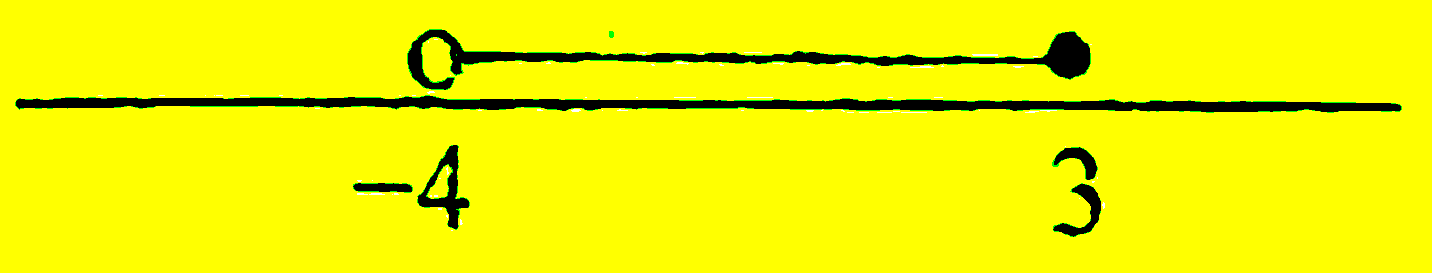
\includegraphics[width=0.3\textwidth]{03.png}

\bigskip 

\noindent 
Eg. $5 x+4 \leq 3 x<6-3 x$

\bigskip 
\begin{tabular}{c|c} 
	$
	\begin{aligned}
		5 x+4 & \leq 3 x \\
		2 x & \leq-4\\
		x & \leq-2
	\end{aligned}
	$
	& 
	$
	\begin{aligned}
		3 x & <6-3 x \\
		6 x & <6 \\
		x & <1
	\end{aligned}
	$
\end{tabular} 

\bigskip 

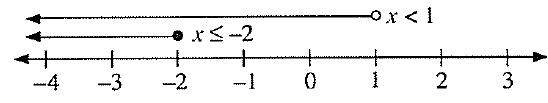
\includegraphics[width=0.4\textwidth]{04.png}

\noindent 
Ans: $x \leq -2$.

\section*{Expansion}

\noindent
Eg.

\noindent
$
\begin{aligned}
	& 2 p-3(p+1) \\
	= & 2 p-3 p-3 \\
	= & -p-3
\end{aligned}
$

\noindent
Eg.

\noindent
$
\begin{aligned}
	& 5 x-(x+1)(2 x-3) \\
	= & 5 x-\left(2 x^2-3 x+2 x-3\right) \\
	= & 5 x-2 x^2+3 x-2 x+3 \\
	= & -2 x^2+6 x+3
\end{aligned}
$

\section*{Factorization and Identities}

\noindent
Factorization of Quadratic Expressions:

\noindent
$
5 x^2+9 x-2
$

\begin{tabular}{c|c|c|}
	$\times$ & \multicolumn{1}{|c}{$5 x$} & $-1$ \\
	\hline$x$ & $5 x^2$ & $-x$ \\
	\cline { 2 - 3 } $2$ & $10 x$ & $-2$ \\
	\hline 
\end{tabular}

\noindent 
$
\therefore \ \ 5 x^2+9 x-2=(5 x-1)(x+2)
$

\bigskip 

\noindent 
Identities:

\bigskip 

\noindent 
1. $(a+b)^2=a^2+2 a b+b^2$

\noindent 
2. $(a-b)^2=a^2-2 a b+b^2$

\noindent 
3. $(a+b)(a-b)=a^2-b^2$

\bigskip 

\noindent 
Common Factorisation Techniques:

\begin{itemize} 
\item Common Factors

Eg. $6 a^3 b-2 a^2 b=2 a^2 b(3 a-1)$

\item Grouping

Eg.

$
\begin{aligned}
	& 6 p^2-3 p q-10 a p+5 a q \\
	& =3 p(2 p-q)-5 a(2 p-q) \\
	& =(3 p-5 a)(2 p-q)
\end{aligned}
$

\item Using Difference of Two Squares

$
\begin{aligned}
	& \text { Eg. } 9 a^2-1 \\
	& =(3a)^2 - (1)^2 \\
	& =(3 a+1)(3 a-1)
\end{aligned}
$

\noindent 
$
\begin{aligned}
	& \text { Eg. } 16 a^4-81 \\
	& =(4a^2+9)(4a^2-9) \\
	& =(4a^2+9)(2a+3)(2a-3)
\end{aligned}
$

\item Combination of methods:

Eg. $3 x^3-12 x y^2$
$=3 x\left(x^2-4 y^2\right)$ common factor
$=3 x(x+2 y)(x-2 y)$ then diff. of 2 squares

Always try common factor first

Eg.

$
\begin{aligned}
	& 4 - p^2 + 6pq - 9q^2  \\
	& =4 - (p^2 - 6pq + 9q^2) \\
	& =(2)^2 - (p-3q)^2 \\
	& =(2+(p-3q))(2-(p-3q)) \\
	& =(2+p-3q)(2-p+3q)
\end{aligned}
$

\end{itemize} 

\newpage 

\section*{Algebraic Fractions}

\noindent 
Eg.

\noindent 
$
\begin{aligned}
	& \frac{x+2}{3}-\frac{x-5}{2}=\frac{2(x+2)}{6}-\frac{3(x-5)}{6} \\	
	& =\frac{2(x+2)-3(x-5)}{6} \\
	& =\frac{2 x+4-3 x+15}{6} \\
	& =\frac{19-x}{6}
\end{aligned}
$

\bigskip 

\noindent 
Eg.

\noindent 
$
\begin{aligned}
	& \frac{5}{x+1}-\frac{2}{x-3} \\
	& =\frac{5(x-3)}{(x+1)(x-3)}-\frac{2(x+1)}{(x-3)(x+1)} \\
	& =\frac{5(x-3)-2(x+1)}{(x+1)(x-3)} \\
	& =\frac{5 x-15-2 x-2}{(x+1)(x-3)} \\
	& =\frac{3 x-17}{(x+2)(x-5)}
\end{aligned}
$

\bigskip 

\noindent 
Eg.

\noindent 
$
\begin{aligned}
	& \frac{5}{3 x}+\frac{2}{x} \\
	& = \frac{5}{3 x}+\frac{6}{3x} \\
	& =\frac{5+6}{3 x} \\
	& =\frac{11}{3 x}
\end{aligned}
$

\bigskip 

\noindent 
Eg. 

\noindent 
$
\begin{aligned}
	& \frac{3}{(x+2)^2}-\frac{4}{x+2} \\
	& =\frac{3}{(x+2)^2}-\frac{4(x+2)}{(x+2)^2} \\	
	& =\frac{3-4(x+2)}{(x+2)^2} \\
	& =\frac{3-4 x-8}{(x+2)^2} \\
	& =\frac{-4 x-5}{(x+2)^2}
\end{aligned}
$

\bigskip 

\noindent 
Eg. 

\noindent 
$
\begin{aligned}
	& \frac{7}{x^2-9}-\frac{1}{x-3} \\
	& =\frac{7}{(x+3)(x-3)}-\frac{1}{x-3} \\
	& =\frac{7}{(x+3)(x-3)}-\frac{x-3}{(x-3)^2} \\	
	& =\frac{7-(x+3)}{(x+3)(x-3)} \\
	& =\frac{7-x-3}{(x+3)(x-3)} \\
	& =\frac{4-x}{(x+3)(x-3)}
\end{aligned}
$

\bigskip 

\noindent 
Eg. 

\noindent 
$\begin{aligned} & \frac{3 x+2}{x^2-4}+\frac{1}{x+2}-\frac{2}{x-2} \\ &= \frac{3 x+2}{(x+2)(x-2)}+\frac{1}{x+2}-\frac{2}{x-2} \\ &= \frac{3 x+2+(x-2)-2(x+2)}{(x+2)(x-2)} \\ &= \frac{3 x+2+x-2-2 x-4}{(x+2)(x-2)} \\ &= \frac{2 x-4}{(x+2)(x-2)} \\ &= \frac{2(x-2)}{(x+2)(x-2)} \\ &= \frac{2}{x+2}\end{aligned}$

\bigskip 

\noindent 
Eg. 

\noindent 
$
\begin{aligned}
	& \frac{9}{x-5}+\frac{3}{5-x} \\
	& =\frac{9}{x-5}-\frac{3}{x-5} \\
	& =\frac{9-3}{x-5} \\
	& =\frac{6}{x-5}
\end{aligned}
$

\bigskip 

\bigskip 

\bigskip 

\bigskip 

\bigskip 

\bigskip 

\bigskip 

\bigskip 

\noindent 
Eg. 

\noindent 
$\begin{aligned} & \frac{2 x}{3 y-8 x}+\frac{11 x}{80 x-30 y} \\ = & \frac{2 x}{3 y-8 x}+\frac{11 x}{-10(3 y-8 x)} \\ = & \frac{2 x}{3 y-8 x}-\frac{11 x}{10(3 y-8 x)} \\ = & \frac{20 x-11 x}{10(3 y-8 x)} \\ = & \frac{9 x}{10(3 y-8 x)}\end{aligned}$

\bigskip 

\noindent 
Eg. 

\noindent 
$\begin{aligned} & \frac{4}{x^2-4}+\frac{1}{2-x} \\ = & \frac{4}{(x+2)(x-2)}-\frac{1}{x-2} \\ = & \frac{4-(x+2)}{(x+2)(x-2)} \\ = & \frac{4-x-2}{(x+2)(x-2)} \\ = & \frac{2-x}{(x+2)(x-2)} \\ = & \frac{-x-2)}{(x+2)(x-2)} \\ = & -\frac{1}{x+2}\end{aligned}$

\bigskip 

\noindent 
Eg. 

\noindent 
$\begin{aligned} & \frac{6 p^3}{7 q} \div \frac{2 p}{21 q^2} \\ = & \frac{6 p^3}{7 q} \times \frac{21 q^2}{2 p} \ \ [\text { do cancelling }] \\ = & 9 p^2 q\end{aligned}$

\bigskip 

\noindent 
Eg. 

\noindent 
$\begin{aligned} \frac{4 p q^2+4 p q r}{9 p q r^2+9 p q^2 r} & =\frac{4 p q(q+r)}{9 p q r(r+q)} \\ & =\frac{4}{9 r}\end{aligned}$

\bigskip 

\bigskip 

\bigskip 

\bigskip 

\bigskip 

\bigskip 

\noindent 
Eg. 

\noindent 
$\begin{aligned} \frac{5 k^2-17 k-12}{5 k^2-10 k-40} & =\frac{(5 k+3)(k-4)}{5\left(k^2-2 k-8\right)} \\ & =\frac{(5 k+3)(k-4)}{5(k-4)(k+2)} \\ & =\frac{5 k+3}{5(k+2)}\end{aligned}$

\bigskip 

\noindent 
Eg. 

\noindent 
$\begin{aligned} & \frac{x y-z^2-x z+y z}{y^2-2 y z+z^2} \div \frac{11}{2 x z+x^2+z^2} \\ & =\frac{x y-x z+y z-z^2}{y^2-2 y z+z^2} \times \frac{2 x z+x^2+z^2}{11} \\ & =\frac{x(y-z)+z(y-z)}{(y-z)^2} \times \frac{(x+z)^2}{11} \\ & =\frac{(x+z)(y-z)}{(y-z)^2} \times \frac{(x+z)^2}{11} \\ & =\frac{(x+z)^3}{11(y-z)}\end{aligned}$


\bigskip 

\noindent 
Eg. 

\noindent 
$\begin{aligned} & \frac{1-\frac{1}{x}}{1-\frac{1}{x^2}} \\ & =\left(1-\frac{1}{x}\right) \div\left(1-\frac{1}{x^2}\right) \\ & =\left(\frac{x-1}{x}\right) \div\left(\frac{x^2-1}{x^2}\right) \\ & =\frac{x-1}{x} \times \frac{x^2}{x^2-1^2} \\ & =\frac{x-1}{x} \times \frac{x^2}{(x+1)(x-1)} \\ & =\frac{x}{x+1}\end{aligned}$

\section*{Making Subject of Formula}

\bigskip 

\noindent 
Eg: Make $a$ the subject

\noindent 
$\begin{aligned} y & = m(x-a)+b \\ y-b & =m(x-a) \\ m(x-a) & =y-b \\ x-a & =\frac{y-b}{m} \\ a & =x-\frac{y-b}{m}\end{aligned}$

\bigskip 

\noindent 
Eg: Make $x$ the subject

\noindent 
$\begin{aligned} a x-b y & =3-2 x \\ a x+2 x & =3+b y \\ x(a+2) & =b y+3 \\ x & =\frac{b y+3}{a+2}\end{aligned}$

\bigskip 

\noindent 
Eg: Make $d$ the subject

\noindent 
$\begin{aligned} T & =0.25 \pi d^2 \\ \pi d^2 & =4 T \\ d^2 & =\frac{4 T}{\pi} \\ d & = \pm \sqrt{\frac{4 T}{\pi}}\end{aligned}$

\noindent
Note the $\pm$ when taking square-roots in this type of question.

\bigskip 

\noindent 
Eg: Make $c$ the subject

\noindent 
$\begin{aligned} d & =\frac{8-c}{c+7} \\ d(c+7) & =8-c \\ c d+7 d & =8-c \\ c d+c & =8-7 d \\ c(d+1) & =8-7 d \\ c & =\frac{8-7 d}{d+1}\end{aligned}$

\bigskip 

\bigskip 

\bigskip 

\bigskip 

\bigskip 

\bigskip 

\bigskip 

\bigskip 

\bigskip 

\noindent 
Eg: Make $q$ the subject

\noindent 
$\begin{aligned} 5 a & =\sqrt{\frac{b^2}{q}-\frac{3 c}{4}} \\ 25 a^2 & =\frac{b^2}{q}-\frac{3 c}{4} \\ \frac{b^2}{q} & =25 a^2+\frac{3 c}{4} \\ \frac{b^2}{q} & =\frac{100 a^2+3 c}{4} \\ \frac{q}{b^2} & =\frac{4}{100 a^2+3 c} \\ q & =\frac{4 b^2}{100 a^2+3 c}\end{aligned}$

\bigskip 

\noindent 
Eg: Make $y$ the subject

\noindent 
$\begin{aligned} \frac{x\left(y z-w^2\right)}{2}-\frac{y}{3} & =6 y \\ 3 x\left(y z-w^2\right)-2 y & =36 y \\ 3 x y z-3 w^2 x-2 y & =36 y \\ 3 x y z-38 y & =3 w^2 x \\ y(3 x z-38) & =3 w^2 x \\ y & =\frac{3 w^2 x}{3 x z-38}\end{aligned}$

\bigskip 

\noindent 
Eg: Make $x$ the subject

\noindent 
$\begin{aligned} p \sqrt{x}+q & =r+s \sqrt{x} \\ p \sqrt{x}-s \sqrt{x} & =r-q \\ \sqrt{x}(p-s) & =r-q \\ \sqrt{x} & =\frac{r-q}{p-s} \\ x & =\left(\frac{r-q}{p-s}\right)^2\end{aligned}$


\section*{Surface Area and Volume of Solids}

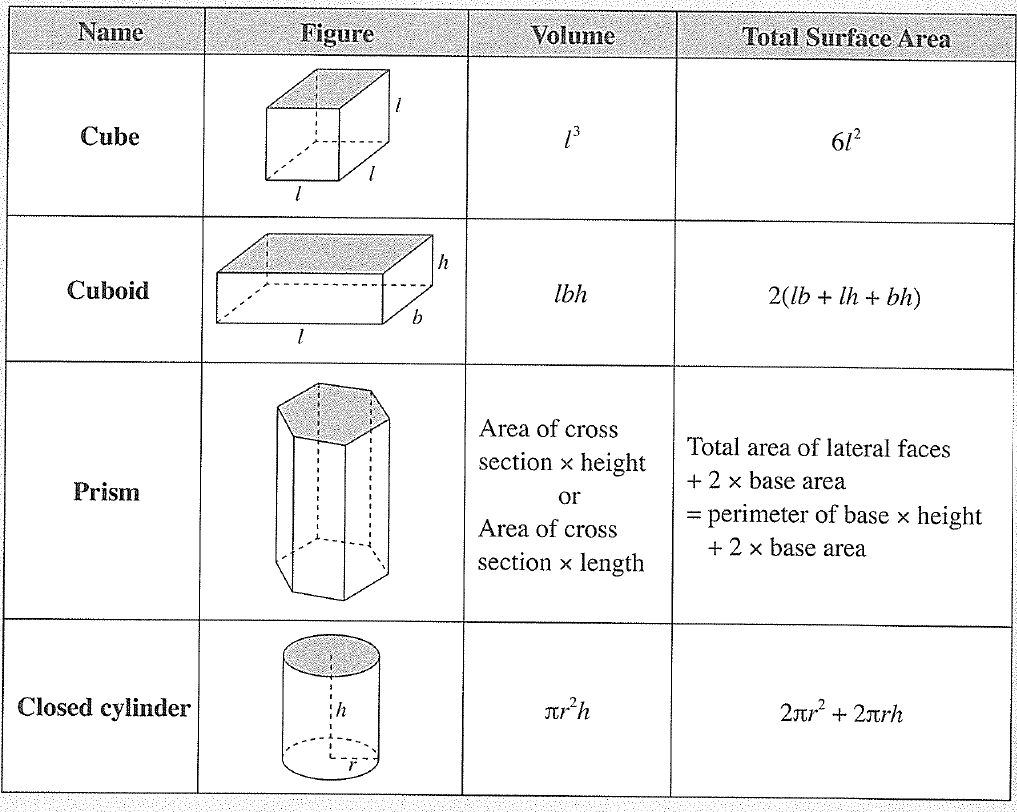
\includegraphics[width=0.5\textwidth]{82.png}

\bigskip 

\noindent 
A pyramid is a solid with a polygonal base and triangles as its slanted faces. Each corner point of a pyramid is called a vertex. The vertex of the pyramid that is above the plane of the polygonal base is known as the apex of the pyramid. The apex is also the point where all the slanted triangular faces meet.

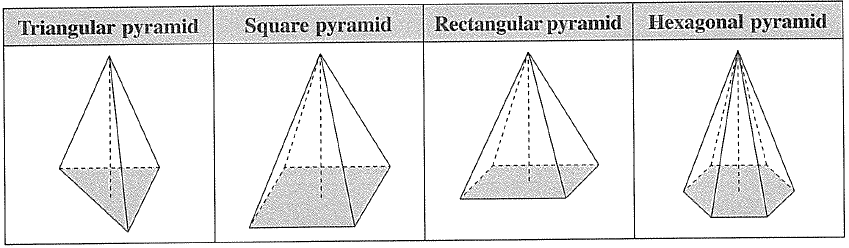
\includegraphics[width=0.48\textwidth]{85.png}

\bigskip 

\noindent 
A pyramid whose apex is vertically above the centre of its base is known as a right pyramid. A pyramid whose apex is not vertically above the centre of its base is known as an oblique pyramid. 

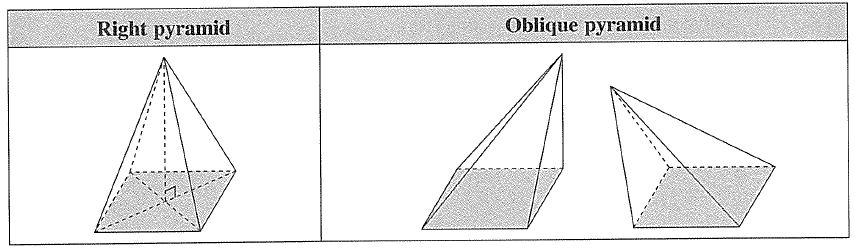
\includegraphics[width=0.48\textwidth]{86.png}

\bigskip 

\noindent 
Surface Area and Volume formulae for Pyramids, Cones, Spheres, Hemispheres:

\bigskip 

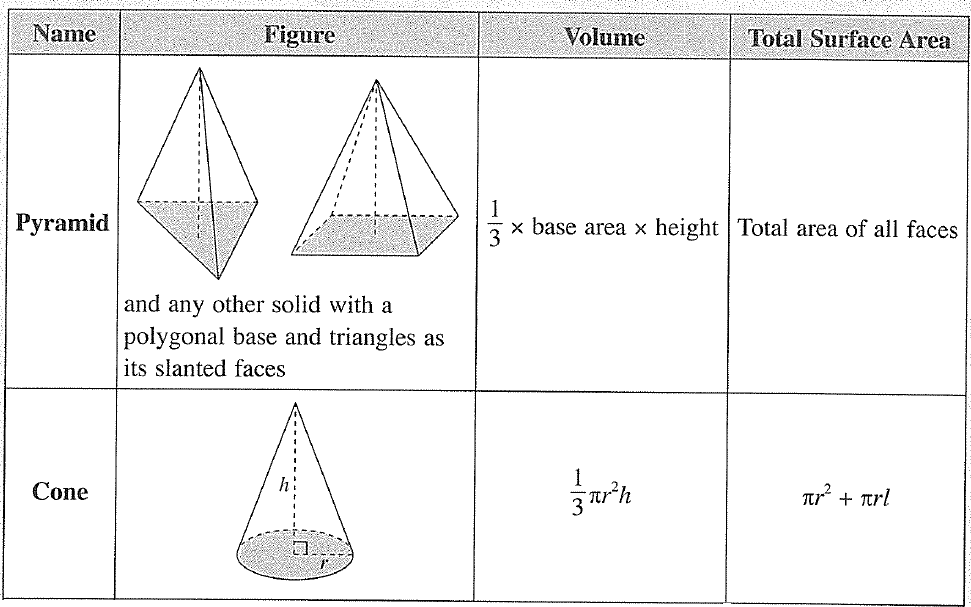
\includegraphics[width=0.48\textwidth]{83.png}

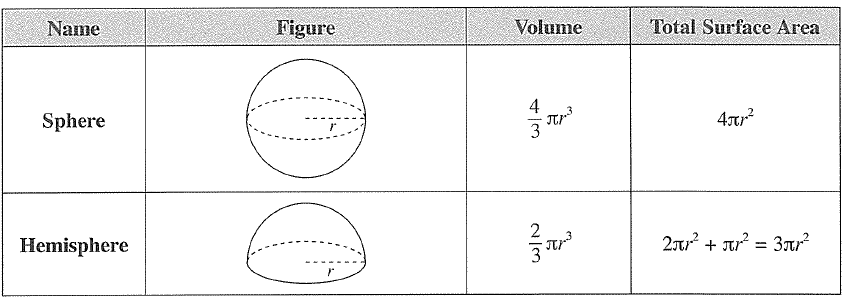
\includegraphics[width=0.48\textwidth]{88.png}

\newpage 

\section*{Pythagoras' Theorem and its converse, Trigonometry}

\noindent 
Pythagoras' Theorem:

\noindent 
For a right-angled $\triangle A B C$,
$$
a^2+b^2=c^2
$$
where $c$ is the length of the hypotenuse.

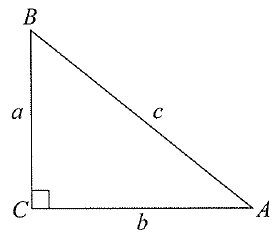
\includegraphics[width=0.25\textwidth]{100.png}

\bigskip 

\noindent 
Converse of Pythagoas' Theorem:

\noindent 
If in a  $\triangle A B C$, we have  $a^2+b^2=c^2$,
then it follows that $\triangle A B C$ is a right-angled triangle with $\angle BCA = 90^{\circ}$

\bigskip 

\noindent 
Trigonometric Ratios of an Acute Angle:
$$
\begin{aligned}
	& \sin \theta=\frac{\text { opposite }}{\text { hypotenuse }}=\frac{a}{c} \\
	& \cos \theta=\frac{\text { adjacent }}{\text { hypotenuse }}=\frac{b}{c} \\
	& \tan \theta=\frac{\text { opposite }}{\text { adjacent }}=\frac{a}{b}
\end{aligned}
$$

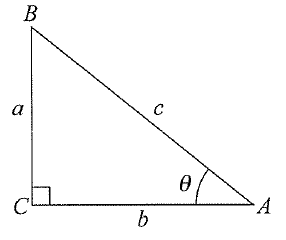
\includegraphics[width=0.25\textwidth]{101.png}

\bigskip 

\noindent 
Obtuse Angles:
$$
\begin{aligned}
	& \text{If} \ x+y=180^{\circ} \ , \ \text{then} \\
	& \sin y=\sin \left(180^{\circ}-x\right)=\sin x \\
	& \cos y=\cos \left(180^{\circ}-x\right)=-\cos x \\
	& \tan y=\tan \left(180^{\circ}-x\right)=-\tan x
\end{aligned}
$$

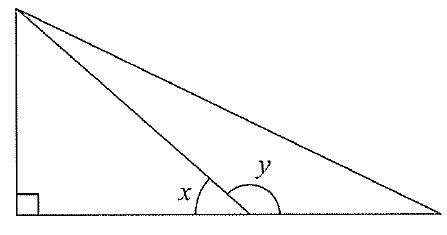
\includegraphics[width=0.25\textwidth]{103.png}

\bigskip

\noindent 
Angles of Elevation and Depression:

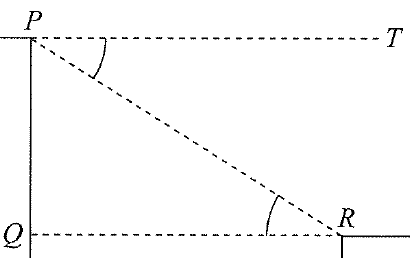
\includegraphics[width=0.3\textwidth]{105.png}

\bigskip

\noindent 
Assume that $QR$ is level ground, and $PT$ is a line parallel to $QR$.

\noindent
$\angle P R Q$ is known as the angle of elevation of $P$ from $R$.

\noindent
$\angle T P R$ is known as the angle of depression of $R$ from $P$.

\noindent
By alternate angles,

\noindent
Angle of elevation of $P$ from $R$, $\angle P R Q=$ Angle of depression of $R$ from $P$, $\angle T P R$.

\end{document}


